\section{How it works}
\label{sec_how_it_works}

\begin{figure}[t]
\begin{center}
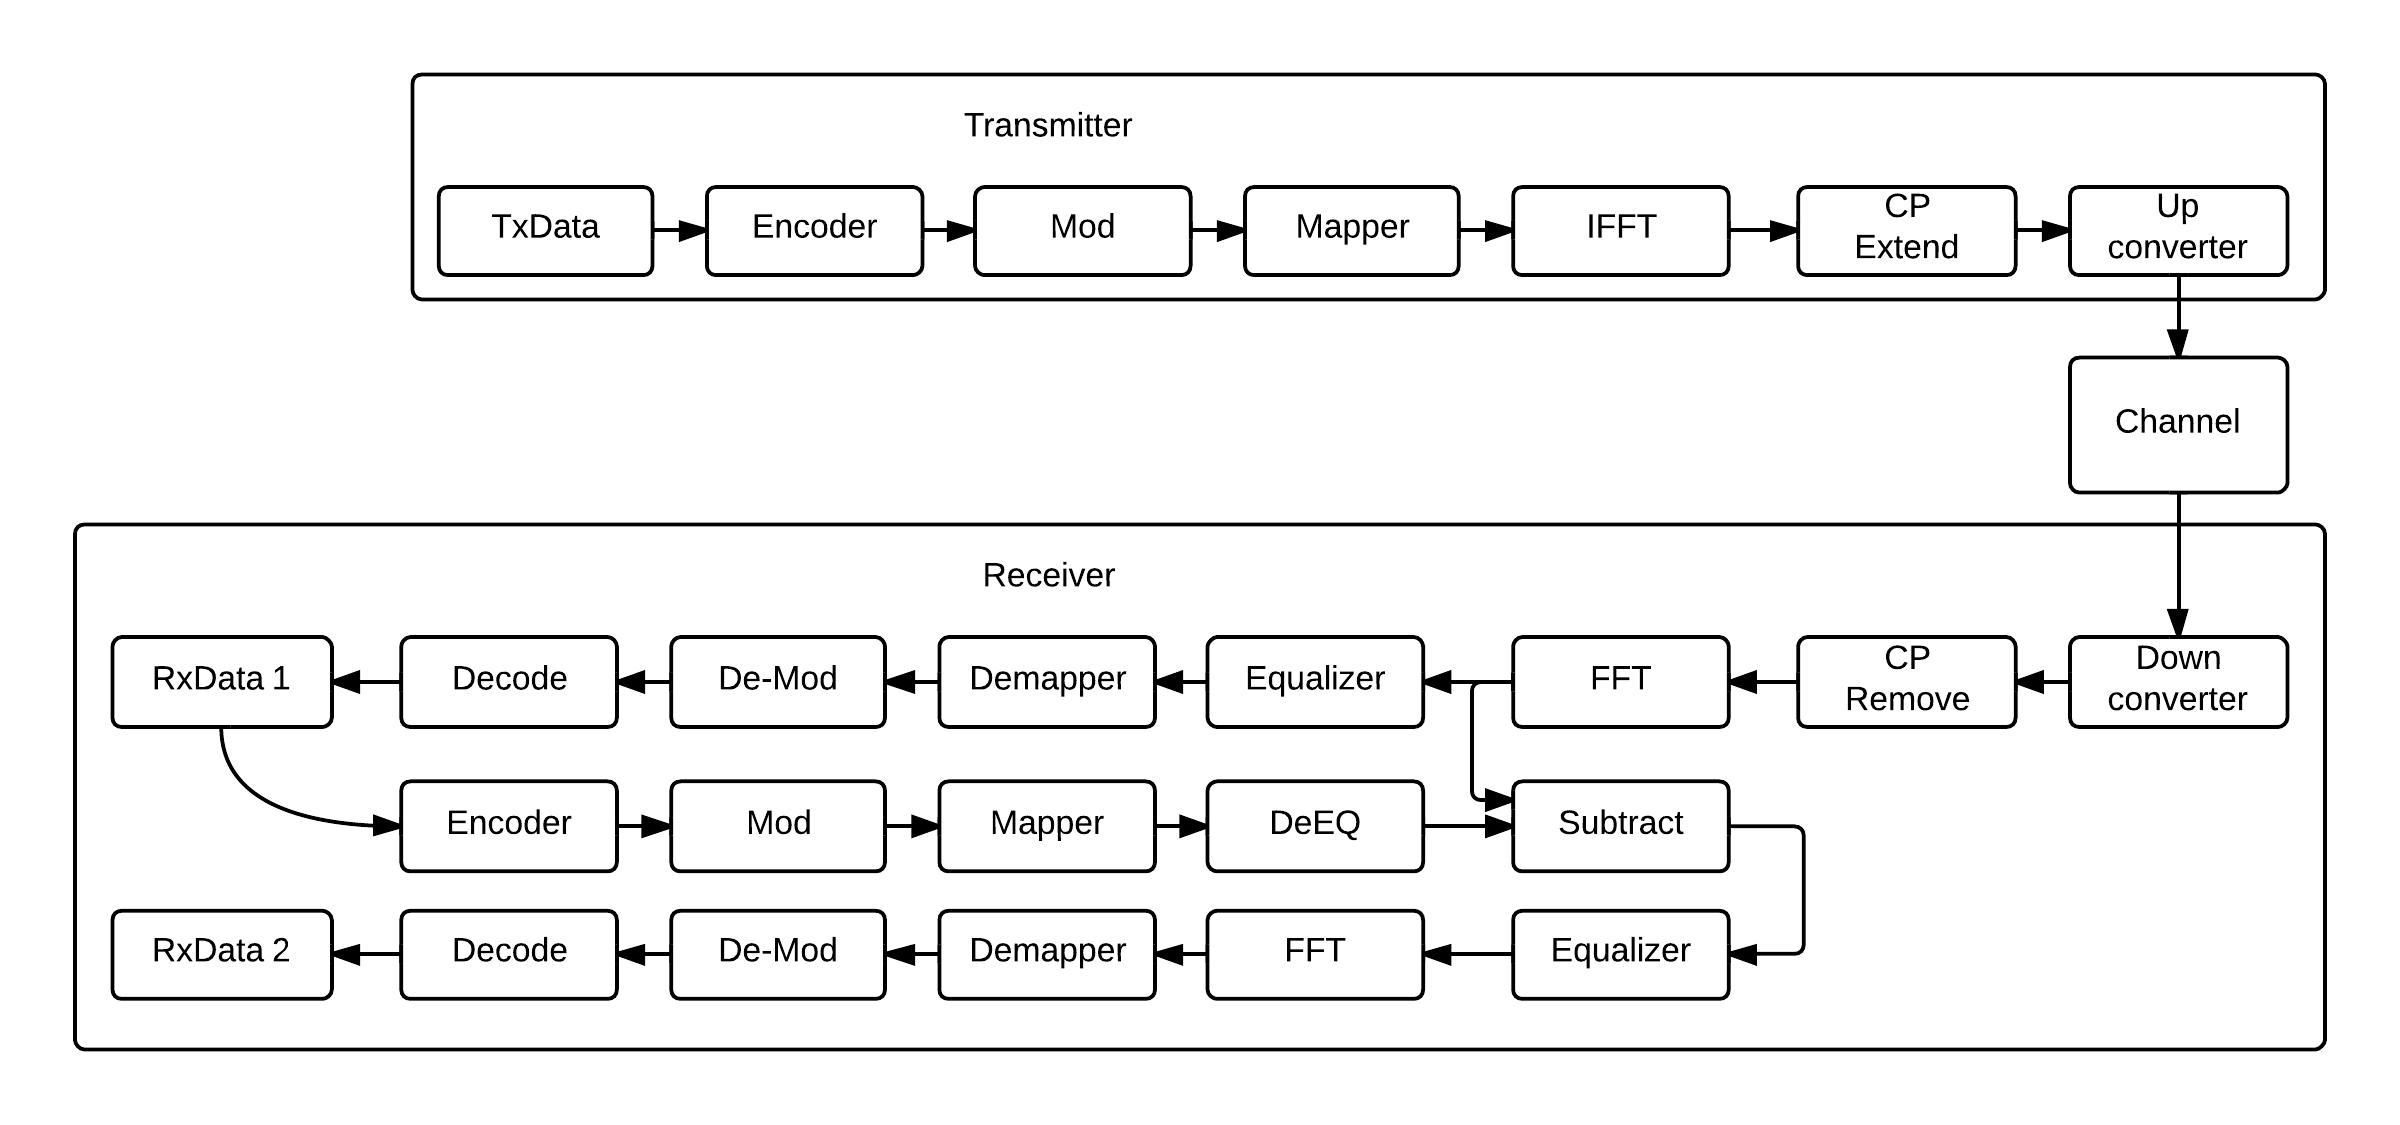
\includegraphics[width=1.0\columnwidth ,angle=0]{figure/systemArch.png}
\caption{simulation architecture}
\label{fig_sys_arch}
\end{center}
\end{figure}

The physical layer simulation is constructed by the system architecture 
shown in Fig.~\ref{fig_sys_arch}.
In this system, the receiver can only extract two layers of multiplexed data.

The system architecture is build with following functional blocks. 1)TxData 
generator: generates binary random bits for transmission, 2)Encoder: encode 
the data by convolutional coding method, 3)Modulator: modulates bits into
symbols, 4)IFFT: maps the frequency domain signals to time domain samples,
5)Cyclic Prefix: appending cyclic prefix, 6)Channel: implement white noise
and multipath enviornments, 7)Equalizer: to compensate the effect of channel.

Fig.~\ref{fig_pair_mcs} shows the highest order of MCS that the users can
achieve in given BER constraint for different channel condition (note that
axis has minus sign.) Here the BER constraint is set to be $10^{-4}$.

To provide quality service in wireless multiple access
network, it’s essential to make proper scheduling between users
when the resources is limited.
Fig.~\ref{fig_my_schedule} shows the topology of
12 users are randomly scattered in 2800 square meter plane.
Each user has to transmit at least once and we have to schedule all users 
in 6 resource blocks with 2 users in each with no overlapping.
Fig.~\ref{fig_my_schedule} shows the schedule result by algorithm~\ref{alg_my}
Pairs of users are painted with different color.

{
\begin{algorithm}[t]
\setcounter{lines}{0}

\algline \textbf{Input}: a set of user equipments, i.e. $\mathbf{V}$

\algline \textbf{Initial}: $CS \leftarrow \varnothing$ \textbackslash\textbackslash schedule set

\algline Sort UEs by its pathloss increasingly.

\textbf{\quad{}\quad{}}$\mathbf{V'} = \{[v_1\medspace v_2 ... v_n] | PL(v_i) \leq PL(v_j) \forall i < j\}$

\algline \textbf{While } $\mathbf{V'}$ is not empty

\algline \textbf{\quad{}} $u = \mathbf{V'}.first()$ \textbackslash\textbackslash select the first element

\algline \textbf{\quad{}For } $r \in \mathbf{V'},\medspace r\neq u$

\algline \textbf{\quad{}}\textbf{\quad{}If } $pair(u,\medspace r)$ is feasible for given constraint

\algline \textbf{\quad{}}\textbf{\quad{}}\textbf{\quad{}} $\mathbf{M} =pair(u,\medspace r).getMCS()$ \textbackslash\textbackslash feasible MCSs

\algline \textbf{\quad{}}\textbf{\quad{}}\textbf{\quad{}For } $W_{m}, m\in \textbf{M}$

\algline \textbf{\quad{}}\textbf{\quad{}}\textbf{\quad{}}\textbf{\quad{}If } $W_{m} > best$

\algline \textbf{\quad{}}\textbf{\quad{}}\textbf{\quad{}}\textbf{\quad{}}\textbf{\quad{}} $best \leftarrow W_{m}$

\algline \textbf{\quad{}}\textbf{\quad{}}\textbf{\quad{}}\textbf{\quad{}}\textbf{\quad{}} $r' \leftarrow r$

\algline \textbf{\quad{}}\textbf{\quad{}}\textbf{\quad{}}\textbf{\quad{}End If}

\algline \textbf{\quad{}}\textbf{\quad{}}\textbf{\quad{}End For}

\algline \textbf{\quad{}}\textbf{\quad{}End If}

\algline \textbf{\quad{}End For}

\algline \textbf{\quad{}If } $v'$ exists \textbackslash\textbackslash $u$ can form a pair.

\algline \textbf{\quad{}}\textbf{\quad{}} $\mathbf{V'}\leftarrow \mathbf{V'}\backslash \{r', u\}$, $CS \leftarrow CS \bigcup \{r', u\}$

\algline \textbf{\quad{}Else }

\algline \textbf{\quad{}}\textbf{\quad{}} $\mathbf{V'}\leftarrow \mathbf{V'}\backslash \{u\}$, $CS \leftarrow CS \bigcup \{u\}$

\algline \textbf{\quad{}End If }

\algline \textbf{End While}

\algline \textbf{Return} $best,\medspace CS$

\caption{\label{alg_my} Scheduling transmission pairs iteratively}
\end{algorithm}
}

\begin{figure}[t]
\begin{center}
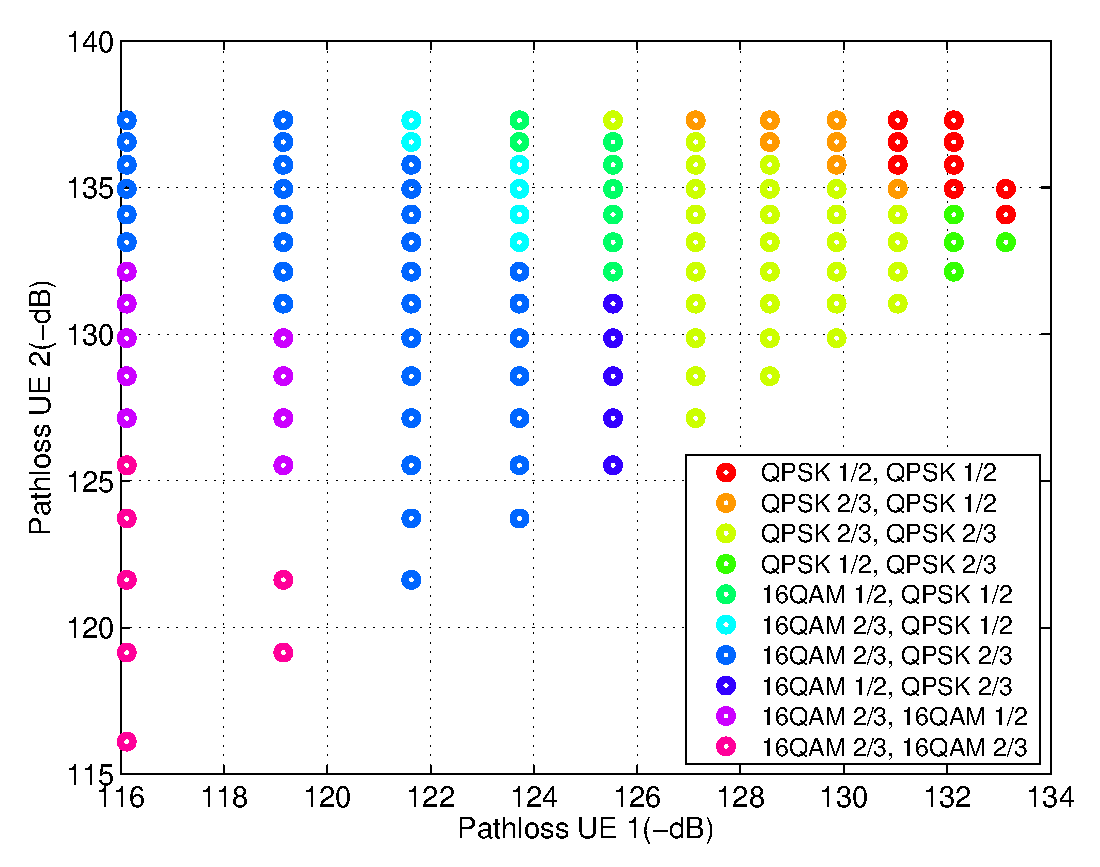
\includegraphics[width=0.9\columnwidth ,angle=0]{figure/pair_mcs.eps}
\caption{MCS supported for BER constraint $10^{-4}$}
\label{fig_pair_mcs}
\end{center}
\end{figure}

\begin{figure}[t]
\begin{center}
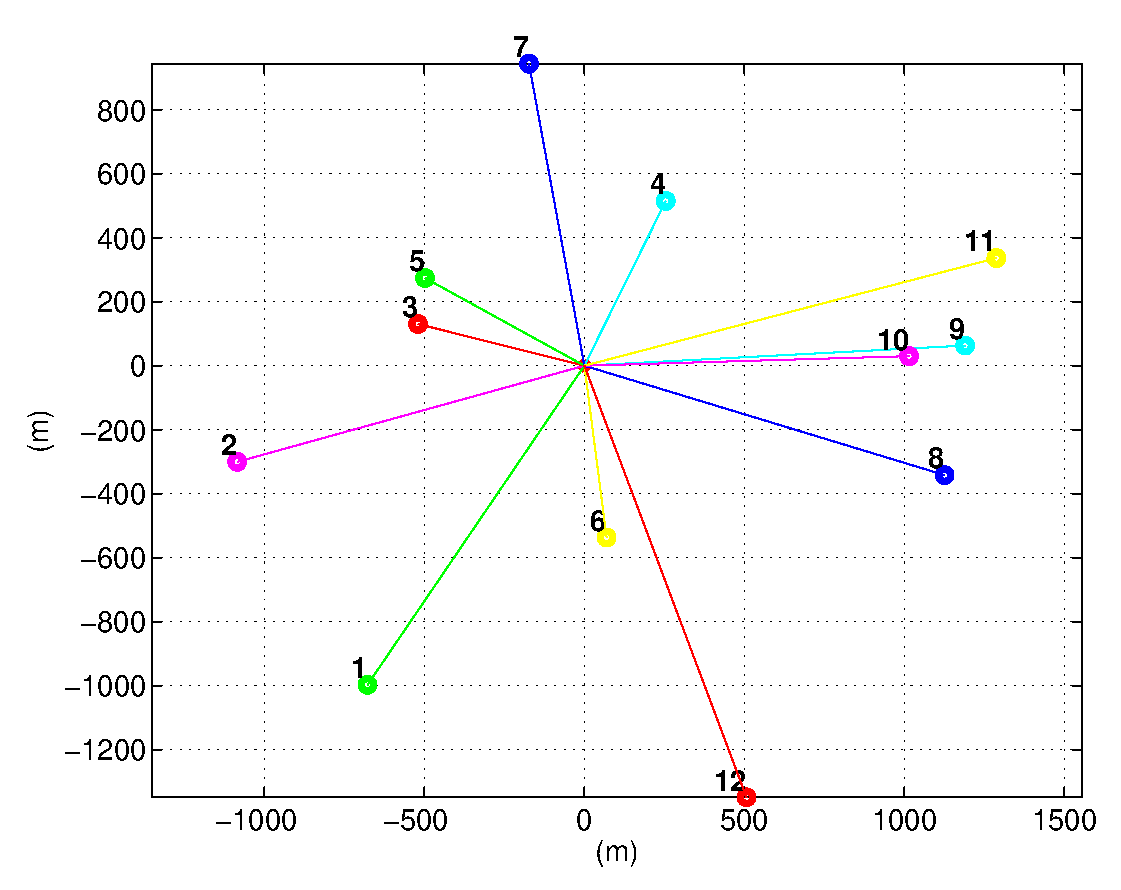
\includegraphics[width=0.9\columnwidth ,angle=0]{figure/my_schedule.eps}
\caption{Scheduled transmission pairs by Alg. 1}
\label{fig_my_schedule}
\end{center}
\end{figure}

%\begin{figure}[t]
%  \centering
%  \subfigure[random caption 1]{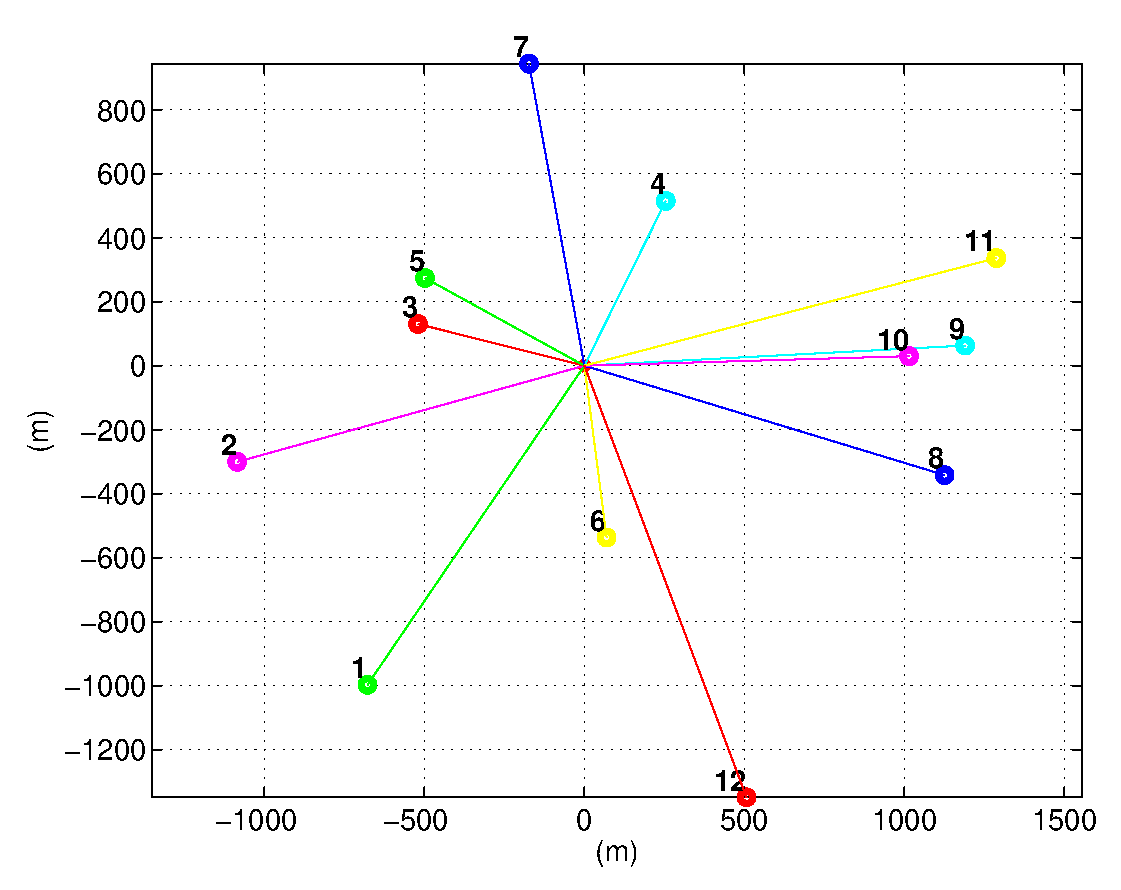
\includegraphics[width=0.45\columnwidth]{figure/my_schedule.eps}}\quad
%  \subfigure[random caption 2]{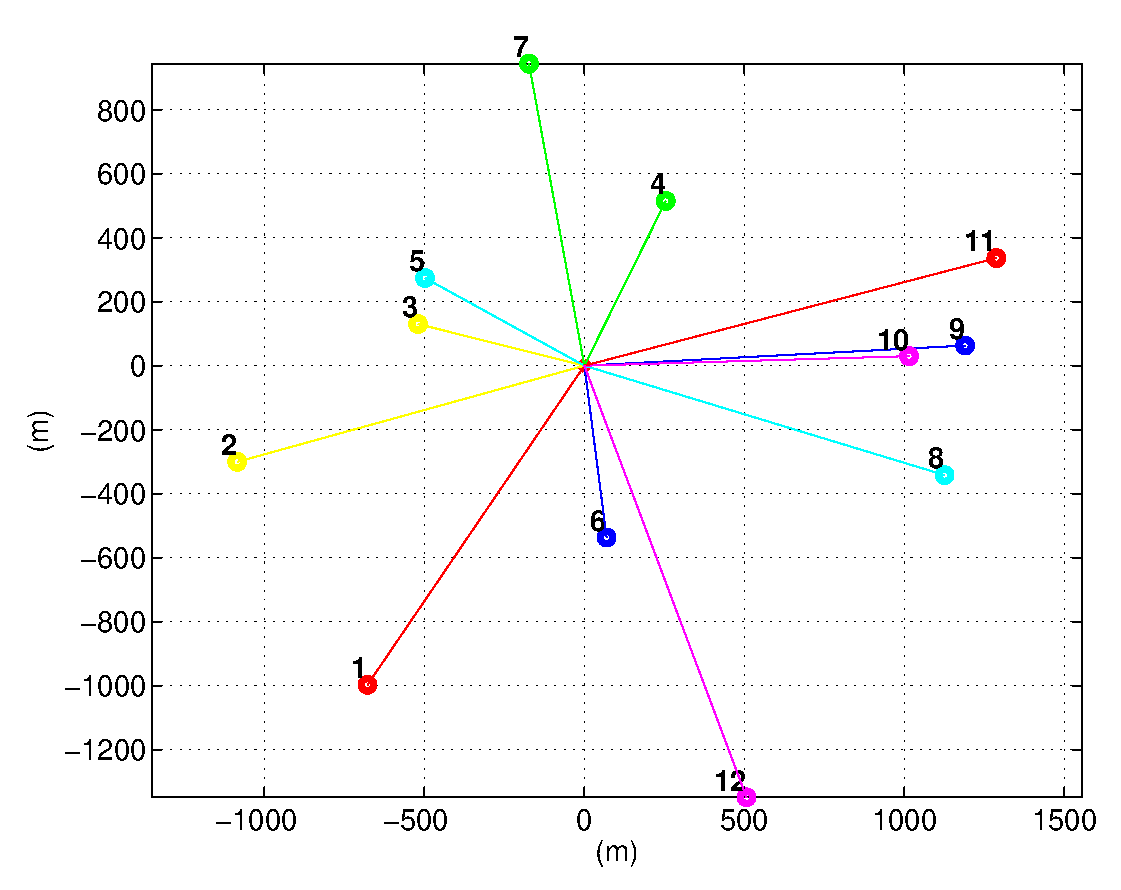
\includegraphics[width=0.45\columnwidth]{figure/schedule_result.eps}}
%\caption{caption}
%\end{figure}

